\documentclass[a4paper,11pt]{article}

\usepackage[utf8]{inputenc}
\usepackage[T1]{fontenc}
% babel french non disponible sur ce système
\usepackage{babel}
\usepackage{geometry}
\geometry{margin=20mm, top=25mm, bottom=25mm}
\usepackage{tikz}
\usetikzlibrary{patterns, arrows.meta, decorations.markings, calc, positioning}
\usepackage{siunitx}
\sisetup{per-mode=symbol}
\usepackage{booktabs}
\usepackage{array}
\usepackage{xcolor}
\usepackage{fancyhdr}
\usepackage{amsmath}
\usepackage{enumitem}
\usepackage{tabularx}
\usepackage{float}

% Couleurs
\definecolor{cotbleu}{HTML}{2563EB}
\definecolor{cotrouge}{HTML}{DC2626}
\definecolor{cotvert}{HTML}{16A34A}
\definecolor{graphitegris}{HTML}{4B5563}
\definecolor{coneint}{HTML}{FCD34D}
\definecolor{fondgris}{HTML}{F3F4F6}

% En-tête / pied de page
\pagestyle{fancy}
\fancyhf{}
\lhead{\small\textsc{Loupe Compton --- Cône Graphite}}
\rhead{\small Plan technique détaillé}
\cfoot{\thepage/\pageref{LastPage}}
\renewcommand{\headrulewidth}{0.4pt}

\usepackage{lastpage}

\title{%
  \vspace{-1cm}
  {\Large\textsc{Plan Technique Détaillé}}\\[4pt]
  {\LARGE\bfseries Cône Concentrateur Graphite}\\[4pt]
  {\large Loupe Compton pour rayons X --- Configuration optimale}\\[2pt]
  {\normalsize $P_C^{\text{fwd}} = \SI{20.6}{\percent}$ à \SI{50}{\keV}}
}
\author{}
\date{Février 2026}

\begin{document}
\maketitle
\thispagestyle{fancy}

% ============================================================
\section{Identification de la pièce}
% ============================================================

\begin{table}[H]
\centering
\begin{tabular}{@{}l l@{}}
\toprule
\textbf{Désignation}   & Cône concentrateur Compton \\
\textbf{Référence}      & LC-GRA-001 \\
\textbf{Matériau}        & Graphite isostatique haute densité \\
\textbf{Grade recommandé}& Poco EDM-3, Toyo Tanso IG-11, ou SGL R8710 \\
\textbf{Granulométrie}   & $< \SI{10}{\micro\meter}$ (grain fin) \\
\textbf{Densité requise} & $\rho \geq \SI{1.80}{\gram\per\centi\meter\cubed}$ (nominale : \SI{2.26}{\gram\per\centi\meter\cubed}) \\
\textbf{Masse estimée}   & $\approx \SI{160}{\gram}$ \\
\textbf{Quantité}        & 1 (prototype) \\
\bottomrule
\end{tabular}
\end{table}

% ============================================================
\section{Vue en coupe longitudinale (plan de symétrie)}
% ============================================================

\begin{figure}[H]
\centering
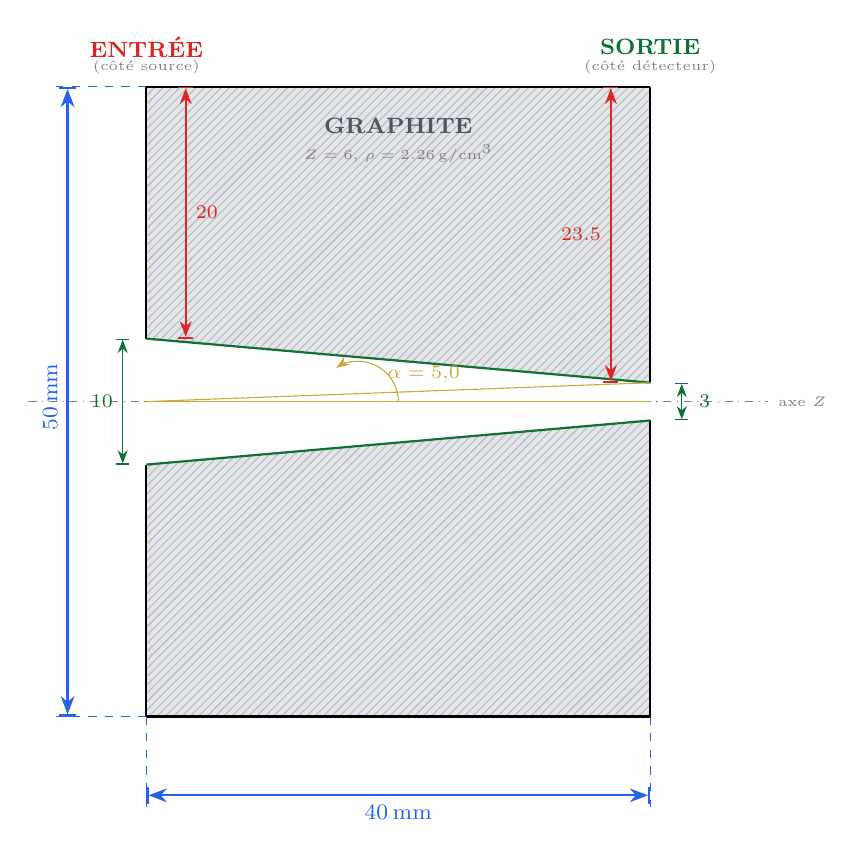
\begin{tikzpicture}[>=Stealth, scale=1, every node/.style={font=\small}]

  % Échelle : 1mm = 0.16 cm sur le dessin (ajusté pour tenir sur la page)
  \pgfmathsetmacro{\s}{0.16}  % scale factor mm -> cm
  
  % Dimensions en mm
  \pgfmathsetmacro{\L}{40}      % longueur
  \pgfmathsetmacro{\Rext}{25}   % rayon extérieur
  \pgfmathsetmacro{\Rin}{5}     % rayon intérieur entrée
  \pgfmathsetmacro{\Rout}{1.5}  % rayon intérieur sortie
  
  % Coordonnées converties
  \pgfmathsetmacro{\Lc}{\L*\s}
  \pgfmathsetmacro{\Rc}{\Rext*\s}
  \pgfmathsetmacro{\Ric}{\Rin*\s}
  \pgfmathsetmacro{\Roc}{\Rout*\s}

  % Corps graphite (hachures)
  % Demi-coupe supérieure
  \fill[graphitegris!15] (0,\Ric) -- (0,\Rc) -- (\Lc,\Rc) -- (\Lc,\Roc) -- cycle;
  \fill[graphitegris!15] (0,-\Ric) -- (0,-\Rc) -- (\Lc,-\Rc) -- (\Lc,-\Roc) -- cycle;
  
  % Hachures
  \fill[pattern=north east lines, pattern color=graphitegris!40] 
    (0,\Ric) -- (0,\Rc) -- (\Lc,\Rc) -- (\Lc,\Roc) -- cycle;
  \fill[pattern=north east lines, pattern color=graphitegris!40] 
    (0,-\Ric) -- (0,-\Rc) -- (\Lc,-\Rc) -- (\Lc,-\Roc) -- cycle;

  % Contour extérieur
  \draw[thick] (0,\Rc) -- (\Lc,\Rc);
  \draw[thick] (0,-\Rc) -- (\Lc,-\Rc);
  \draw[thick] (0,\Rc) -- (0,\Ric);
  \draw[thick] (0,-\Rc) -- (0,-\Ric);
  \draw[thick] (\Lc,\Rc) -- (\Lc,\Roc);
  \draw[thick] (\Lc,-\Rc) -- (\Lc,-\Roc);
  
  % Contour intérieur (cône)
  \draw[thick, cotvert!70!black] (0,\Ric) -- (\Lc,\Roc);
  \draw[thick, cotvert!70!black] (0,-\Ric) -- (\Lc,-\Roc);

  % Axe de symétrie
  \draw[dash dot, thin, gray] (-1.5,0) -- (\Lc+1.5,0) node[right, font=\tiny, gray] {axe $Z$};

  % ---- COTES ----
  
  % Longueur totale (en bas)
  \pgfmathsetmacro{\cotY}{-\Rc-1.0}
  \draw[cotbleu, |<->|, thick] (0,\cotY) -- node[below, font=\footnotesize\bfseries, cotbleu] {\SI{40}{\milli\meter}} (\Lc,\cotY);
  \draw[cotbleu, thin, dashed] (0,-\Rc) -- (0,\cotY-0.15);
  \draw[cotbleu, thin, dashed] (\Lc,-\Rc) -- (\Lc,\cotY-0.15);

  % Diamètre extérieur (à gauche)
  \pgfmathsetmacro{\cotX}{-1.0}
  \draw[cotbleu, |<->|, thick] (\cotX,-\Rc) -- node[left, font=\footnotesize\bfseries, cotbleu, rotate=90, anchor=south] {$\varnothing$ \SI{50}{\milli\meter}} (\cotX,\Rc);
  \draw[cotbleu, thin, dashed] (0,\Rc) -- (\cotX-0.15,\Rc);
  \draw[cotbleu, thin, dashed] (0,-\Rc) -- (\cotX-0.15,-\Rc);

  % Diamètre intérieur entrée
  \pgfmathsetmacro{\cotXin}{-0.3}
  \draw[cotvert!70!black, |<->|] (\cotXin,-\Ric) -- node[left, font=\scriptsize, cotvert!70!black] {$\varnothing$ \SI{10}{}} (\cotXin,\Ric);

  % Diamètre intérieur sortie
  \pgfmathsetmacro{\cotXout}{\Lc+0.4}
  \draw[cotvert!70!black, |<->|] (\cotXout,-\Roc) -- node[right, font=\scriptsize, cotvert!70!black] {$\varnothing$ \SI{3}{}} (\cotXout,\Roc);

  % Épaisseur paroi entrée (côté supérieur)
  \pgfmathsetmacro{\parX}{0.5}
  \draw[cotrouge, |<->|, semithick] (\parX,\Ric) -- node[right, font=\scriptsize, cotrouge] {\SI{20}{}} (\parX,\Rc);

  % Épaisseur paroi sortie (côté supérieur)
  \pgfmathsetmacro{\parXs}{\Lc-0.5}
  \draw[cotrouge, |<->|, semithick] (\parXs,\Roc) -- node[left, font=\scriptsize, cotrouge] {\SI{23.5}{}} (\parXs,\Rc);

  % Demi-angle
  \draw[coneint!80!black, thin] (0,0) -- (\Lc,0);
  \draw[coneint!80!black, thin] (0,0) -- (\Lc,\Roc);
  \draw[coneint!80!black, ->] ({\Lc*0.5},0) arc[start angle=0, end angle={atan(\Roc/\Lc)*180/3.14159}, radius={\Lc*0.5*\s}];
  \node[coneint!80!black, font=\scriptsize] at ({\Lc*0.55},0.35) {$\alpha = 5{,}0°$};

  % Labels
  \node[font=\footnotesize\bfseries, cotrouge] at (0, \Rc+0.5) {ENTRÉE};
  \node[font=\tiny, gray] at (0, \Rc+0.25) {(côté source)};
  \node[font=\footnotesize\bfseries, cotvert!70!black] at (\Lc, \Rc+0.5) {SORTIE};
  \node[font=\tiny, gray] at (\Lc, \Rc+0.25) {(côté détecteur)};

  % Label matériau
  \node[font=\footnotesize\bfseries, graphitegris] at ({\Lc/2}, {\Rc-0.5}) {GRAPHITE};
  \node[font=\tiny, gray] at ({\Lc/2}, {\Rc-0.85}) {$Z=6$, $\rho = \SI{2.26}{\gram/\centi\meter^3}$};

\end{tikzpicture}
\caption{Vue en coupe longitudinale du cône concentrateur. Les cotes sont en millimètres sauf indication contraire. L'alésage interne est conique avec un demi-angle $\alpha = 5{,}0°$.}
\label{fig:coupe_long}
\end{figure}

% ============================================================
\section{Vues en coupe transversale}
% ============================================================

\begin{figure}[H]
\centering
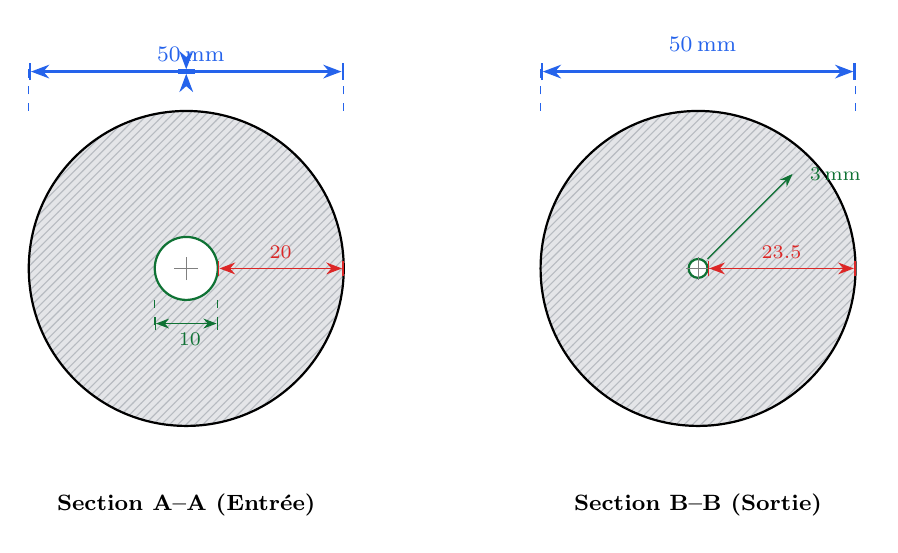
\begin{tikzpicture}[>=Stealth, every node/.style={font=\small}]

  % --- Section A-A (Entrée) ---
  \begin{scope}[shift={(0,0)}]
    % Graphite
    \fill[graphitegris!15] (0,0) circle (2.0);
    \fill[pattern=north east lines, pattern color=graphitegris!40] (0,0) circle (2.0);
    % Alésage
    \fill[white] (0,0) circle (0.4);
    \draw[thick] (0,0) circle (2.0);
    \draw[thick, cotvert!70!black] (0,0) circle (0.4);
    
    % Centre
    \draw[thin, gray] (-0.15,0) -- (0.15,0);
    \draw[thin, gray] (0,-0.15) -- (0,0.15);
    
    % Cotes
    \draw[cotbleu, |<->|, thick] (0,2.5) -- node[above, font=\footnotesize\bfseries, cotbleu] {$\varnothing$ \SI{50}{\milli\meter}} (0,2.5);
    \draw[cotbleu, |<->|, thick] (-2.0,2.5) -- (2.0,2.5);
    \draw[cotbleu, thin, dashed] (-2.0,2.0) -- (-2.0,2.6);
    \draw[cotbleu, thin, dashed] (2.0,2.0) -- (2.0,2.6);
    
    \draw[cotvert!70!black, |<->|] (-0.4,-0.7) -- node[below, font=\scriptsize, cotvert!70!black] {$\varnothing$ \SI{10}{}} (0.4,-0.7);
    \draw[cotvert!70!black, thin, dashed] (-0.4,-0.4) -- (-0.4,-0.8);
    \draw[cotvert!70!black, thin, dashed] (0.4,-0.4) -- (0.4,-0.8);
    
    % Paroi
    \draw[cotrouge, |<->|, semithick] (0.4,0) -- node[above, font=\scriptsize, cotrouge] {\SI{20}{}} (2.0,0);
    
    \node[font=\footnotesize\bfseries] at (0,-3.0) {Section A--A (Entrée)};
  \end{scope}

  % --- Section B-B (Sortie) ---
  \begin{scope}[shift={(6.5,0)}]
    % Graphite
    \fill[graphitegris!15] (0,0) circle (2.0);
    \fill[pattern=north east lines, pattern color=graphitegris!40] (0,0) circle (2.0);
    % Alésage (petit)
    \fill[white] (0,0) circle (0.12);
    \draw[thick] (0,0) circle (2.0);
    \draw[thick, cotvert!70!black] (0,0) circle (0.12);
    
    % Centre
    \draw[thin, gray] (-0.15,0) -- (0.15,0);
    \draw[thin, gray] (0,-0.15) -- (0,0.15);
    
    % Cotes
    \draw[cotbleu, |<->|, thick] (-2.0,2.5) -- (2.0,2.5);
    \draw[cotbleu, thin, dashed] (-2.0,2.0) -- (-2.0,2.6);
    \draw[cotbleu, thin, dashed] (2.0,2.0) -- (2.0,2.6);
    \node[cotbleu, font=\footnotesize\bfseries] at (0,2.85) {$\varnothing$ \SI{50}{\milli\meter}};
    
    % Annotation alésage
    \draw[cotvert!70!black, ->] (0.12,0.12) -- (1.2,1.2) node[right, font=\scriptsize, cotvert!70!black] {$\varnothing$ \SI{3}{\milli\meter}};
    
    % Paroi
    \draw[cotrouge, |<->|, semithick] (0.12,0) -- node[above, font=\scriptsize, cotrouge] {\SI{23.5}{}} (2.0,0);
    
    \node[font=\footnotesize\bfseries] at (0,-3.0) {Section B--B (Sortie)};
  \end{scope}

\end{tikzpicture}
\caption{Vues en coupe transversale aux deux extrémités. Le diamètre extérieur est constant ($\varnothing\,\SI{50}{\milli\meter}$). L'alésage diminue de $\varnothing\,\SI{10}{}$ à $\varnothing\,\SI{3}{\milli\meter}$.}
\label{fig:coupe_trans}
\end{figure}

% ============================================================
\section{Tableau de cotation}
% ============================================================

\begin{table}[H]
\centering
\caption{Dimensions et tolérances de la pièce.}
\label{tab:cotes}
\renewcommand{\arraystretch}{1.25}
\begin{tabular}{@{} l c c c @{}}
\toprule
\textbf{Cote} & \textbf{Nominale} & \textbf{Tolérance} & \textbf{Remarque} \\
\midrule
Diamètre extérieur          & \SI{50.0}{\milli\meter}  & $\pm\,\SI{0.1}{}$ & Cylindrique constant \\
Longueur totale              & \SI{40.0}{\milli\meter}  & $\pm\,\SI{0.2}{}$ & --- \\
Alésage entrée ($\varnothing$) & \SI{10.0}{\milli\meter} & $\pm\,\SI{0.05}{}$ & --- \\
Alésage sortie ($\varnothing$) & \SI{3.0}{\milli\meter}  & $\pm\,\SI{0.05}{}$ & --- \\
Demi-angle du cône interne   & $5{,}0°$                 & $\pm\,0{,}2°$     & Critique pour la géométrie \\
Épaisseur paroi (entrée)     & \SI{20.0}{\milli\meter}  & (déduite)          & $= (D_{\text{ext}} - D_{\text{int,e}})/2$ \\
Épaisseur paroi (sortie)     & \SI{23.5}{\milli\meter}  & (déduite)          & $= (D_{\text{ext}} - D_{\text{int,s}})/2$ \\
\midrule
\multicolumn{4}{@{}l}{\textit{État de surface}} \\
Surface intérieure (cône)    & \multicolumn{2}{c}{$R_a < \SI{3.2}{\micro\meter}$} & Poli si possible \\
Surface extérieure           & \multicolumn{2}{c}{$R_a < \SI{6.3}{\micro\meter}$} & Usinage standard \\
\bottomrule
\end{tabular}
\end{table}

% ============================================================
\section{Filtre passe-haut en cuivre}
% ============================================================

Le filtre est une pièce séparée, placée entre la sortie du tube MiniX et l'entrée du cône.

\begin{table}[H]
\centering
\caption{Spécifications du filtre Cu.}
\label{tab:filtre}
\renewcommand{\arraystretch}{1.2}
\begin{tabular}{@{} l l @{}}
\toprule
\textbf{Paramètre} & \textbf{Valeur} \\
\midrule
Matériau         & Cuivre (Cu), feuille laminée \\
Épaisseur        & \SI{25}{\micro\meter} \\
Diamètre utile   & $\geq \SI{12}{\milli\meter}$ \\
Fournisseurs     & Goodfellow, Alfa Aesar \\
Position         & Sortie du tube, collée ou pincée sur anneau support \\
\midrule
\multicolumn{2}{@{}l}{\textit{Effet sur le spectre}} \\
Coupure          & $E < \SI{15}{\keV}$ fortement atténué \\
Énergie effective & $\sim \SI{35}{}$ à \SI{50}{\keV} \\
Rôle             & Supprimer la zone où $\sigma_{\text{ph}} > \sigma_C$ dans le graphite \\
\bottomrule
\end{tabular}
\end{table}

% ============================================================
\section{Assemblage et montage}
% ============================================================

\begin{figure}[H]
\centering
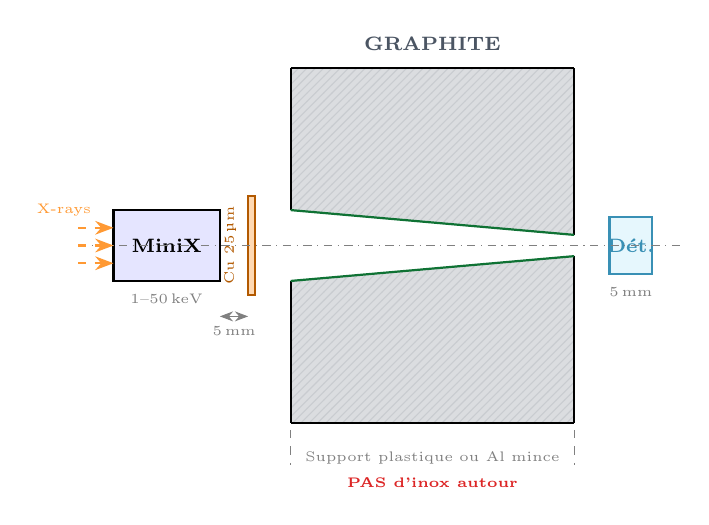
\begin{tikzpicture}[>=Stealth, scale=0.9, every node/.style={font=\small}]

  % Source MiniX
  \fill[blue!10] (-4.5,-0.5) rectangle (-3.0,0.5);
  \draw[thick] (-4.5,-0.5) rectangle (-3.0,0.5);
  \node[font=\scriptsize\bfseries] at (-3.75,0) {MiniX};
  \node[font=\tiny, gray] at (-3.75,-0.75) {1--\SI{50}{\keV}};

  % Filtre Cu
  \fill[orange!30] (-2.6,-0.7) rectangle (-2.5,0.7);
  \draw[thick, orange!70!black] (-2.6,-0.7) rectangle (-2.5,0.7);
  \node[font=\tiny, orange!70!black, rotate=90] at (-2.85,0) {Cu \SI{25}{\micro\meter}};

  % Espace
  \draw[<->, gray, thin] (-3.0,-1.0) -- node[below, font=\tiny, gray] {\SI{5}{\milli\meter}} (-2.6,-1.0);

  % Cône graphite (simplifié)
  \pgfmathsetmacro{\s}{0.1}
  \pgfmathsetmacro{\Lc}{40*\s}
  \pgfmathsetmacro{\Rc}{25*\s}
  \pgfmathsetmacro{\Ric}{5*\s}
  \pgfmathsetmacro{\Roc}{1.5*\s}
  
  \begin{scope}[shift={(-2.0,0)}]
    \fill[graphitegris!20] (0,\Ric) -- (0,\Rc) -- (\Lc,\Rc) -- (\Lc,\Roc) -- cycle;
    \fill[graphitegris!20] (0,-\Ric) -- (0,-\Rc) -- (\Lc,-\Rc) -- (\Lc,-\Roc) -- cycle;
    \fill[pattern=north east lines, pattern color=graphitegris!30] 
      (0,\Ric) -- (0,\Rc) -- (\Lc,\Rc) -- (\Lc,\Roc) -- cycle;
    \fill[pattern=north east lines, pattern color=graphitegris!30] 
      (0,-\Ric) -- (0,-\Rc) -- (\Lc,-\Rc) -- (\Lc,-\Roc) -- cycle;
    \draw[thick] (0,\Rc) -- (\Lc,\Rc);
    \draw[thick] (0,-\Rc) -- (\Lc,-\Rc);
    \draw[thick] (0,\Rc) -- (0,\Ric);
    \draw[thick] (0,-\Rc) -- (0,-\Ric);
    \draw[thick] (\Lc,\Rc) -- (\Lc,\Roc);
    \draw[thick] (\Lc,-\Rc) -- (\Lc,-\Roc);
    \draw[thick, cotvert!70!black] (0,\Ric) -- (\Lc,\Roc);
    \draw[thick, cotvert!70!black] (0,-\Ric) -- (\Lc,-\Roc);
    
    \node[font=\scriptsize\bfseries, graphitegris] at ({\Lc/2},{\Rc+0.35}) {GRAPHITE};
  \end{scope}

  % Détecteur
  \begin{scope}[shift={(2.5,0)}]
    \fill[cyan!10] (0,-0.4) rectangle (0.6,0.4);
    \draw[thick, cyan!70!black] (0,-0.4) rectangle (0.6,0.4);
    \node[font=\scriptsize\bfseries, cyan!70!black] at (0.3,0) {Dét.};
    \node[font=\tiny, gray] at (0.3,-0.65) {\SI{5}{\milli\meter}};
  \end{scope}

  % Axe optique
  \draw[dash dot, thin, gray] (-5,0) -- (3.5,0);

  % Photons
  \foreach \y in {-0.25, 0, 0.25} {
    \draw[->, orange!80, thick, dashed] (-5,\y) -- (-4.5,\y);
  }
  \node[font=\tiny, orange!80] at (-5.2,0.5) {X-rays};

  % Support (indication)
  \draw[thin, gray, dashed] (-2.0,-\Rc-0.1) -- (-2.0,-\Rc-0.6);
  \draw[thin, gray, dashed] (2.0,-\Rc-0.1) -- (2.0,-\Rc-0.6);
  \node[font=\tiny, gray] at (0,-\Rc-0.5) {Support plastique ou Al mince};
  \node[font=\tiny, cotrouge] at (0,-\Rc-0.85) {\textbf{PAS d'inox autour}};

\end{tikzpicture}
\caption{Schéma d'assemblage : tube MiniX $\to$ filtre Cu $\to$ cône graphite $\to$ détecteur. Le cône est maintenu par un support en plastique ou aluminium mince, sans porte-collimateur inox.}
\label{fig:assemblage}
\end{figure}

\subsection*{Contraintes de montage}

\begin{enumerate}[leftmargin=*, itemsep=2pt]
  \item \textbf{Alignement :} l'axe du cône doit être coaxial avec l'axe du faisceau MiniX à $\pm\,0{,}5°$ près. Prévoir un système de centrage par 3~vis à~$120°$ sur le support.
  \item \textbf{Aucun matériau haut-$Z$ autour du cône :} le porte-collimateur inox d'origine doit être retiré ou remplacé par un manchon en PMMA, PTFE ou aluminium mince ($t < \SI{1}{\milli\meter}$).
  \item \textbf{Distance source--entrée :} $\sim \SI{5}{\milli\meter}$, le filtre Cu s'intercale dans cet espace.
  \item \textbf{Distance sortie--détecteur :} aussi faible que possible, $< \SI{5}{\milli\meter}$.
\end{enumerate}

% ============================================================
\section{Performances attendues}
% ============================================================

\begin{table}[H]
\centering
\caption{Bilan photonique à \SI{50}{\keV} pour une paroi de \SI{20}{\milli\meter} de graphite.}
\label{tab:perf}
\renewcommand{\arraystretch}{1.25}
\begin{tabular}{@{} l r l @{}}
\toprule
\textbf{Devenir du photon} & \textbf{Fraction} & \textbf{Statut} \\
\midrule
Transmis sans interaction   & \SI{58.2}{\percent} & Perdu (traverse la paroi) \\
Compton forward (utile)     & \SI{20.6}{\percent} & \textcolor{cotvert}{\textbf{Utile}} \\
Compton arrière             & \SI{20.6}{\percent} & Perdu (rétrodiffusé) \\
Photoélectrique (absorbé)   & \SI{0.6}{\percent}  & Perdu (absorbé) \\
\midrule
Rapport $\sigma_C / \sigma_{\text{ph}}$ & \multicolumn{2}{l}{$\approx 69$ (très favorable)} \\
Perte d'énergie par diffusion & \multicolumn{2}{l}{$\Delta E / E < \SI{5}{\percent}$ (régime Thomson)} \\
\bottomrule
\end{tabular}
\end{table}

\subsection*{Comparaison avec la configuration actuelle}

\begin{table}[H]
\centering
\renewcommand{\arraystretch}{1.2}
\begin{tabular}{@{} l c c c c @{}}
\toprule
\textbf{Configuration} & $E$ (keV) & $t$ (mm) & $P_C^{\text{fwd}}$ & $\sigma_C/\sigma_{\text{ph}}$ \\
\midrule
Cône actuel (graphite 2,1\,mm, 10\,keV) & 10 & 2,1 & \SI{3.0}{\percent} & 0,19 \\
\textbf{Cône optimisé (graphite 20\,mm, 50\,keV)} & \textbf{50} & \textbf{20} & \textbf{\SI{20.6}{\percent}} & \textbf{69} \\
\bottomrule
\end{tabular}
\end{table}

Le gain est d'un \textbf{facteur $\sim 7$} sur le rendement Compton forward, et d'un \textbf{facteur $\sim 360$} sur la sélectivité Compton/photoélectrique.

% ============================================================
\section{Notes de fabrication}
% ============================================================

\begin{enumerate}[leftmargin=*, itemsep=4pt]
  \item \textbf{Brut :} barreau de graphite isostatique $\varnothing\,\SI{55}{} \times \SI{50}{\milli\meter}$ (surcote de \SI{5}{\milli\meter} pour dressage).
  
  \item \textbf{Opération 1 --- Tournage extérieur :}
  dressage des deux faces, chariotage au $\varnothing\,\SI{50}{\milli\meter}$, longueur \SI{40}{\milli\meter}. Outils HSS ou carbure standard. Vitesse de coupe : $V_c \approx \SI{150}{}$ à \SI{300}{\meter/\minute}.

  \item \textbf{Opération 2 --- Perçage pilote :}
  perçage traversant $\varnothing\,\SI{3}{\milli\meter}$ depuis la face de sortie (mandrin de tour).

  \item \textbf{Opération 3 --- Alésage conique :}
  depuis la face d'entrée, chariot orienté à $5°$, alésage progressif de $\varnothing\,\SI{3}{}$ jusqu'à $\varnothing\,\SI{10}{\milli\meter}$ sur \SI{40}{\milli\meter} de profondeur. Alternative~: alésage étagé ($\varnothing\,\SI{4}{}$, $\varnothing\,\SI{6}{}$, $\varnothing\,\SI{8}{}$, $\varnothing\,\SI{10}{}$) puis finition à l'alésoir conique.

  \item \textbf{Opération 4 --- Finition intérieure :}
  polissage léger de la surface conique intérieure ($R_a < \SI{3.2}{\micro\meter}$). Utiliser un mandrin conique garni de papier abrasif fin (grain 400 puis 800).

  \item \textbf{Précautions :}
  \begin{itemize}[itemsep=1pt]
    \item Aspiration des poussières de graphite obligatoire (poussière fine conductrice).
    \item Port d'un masque FFP2 recommandé.
    \item Le graphite est \textbf{non toxique} (contrairement au béryllium).
    \item Pas de lubrification nécessaire (usinage à sec).
  \end{itemize}
\end{enumerate}

\end{document}
